\section{Introduction}
\label{sec:intro}

RGB-D images are increasingly common as sensor technology becomes more widely available and affordable. These images can be used to reconstruct the 3D shapes of objects as well as their surface properties. The better the quality of the depth component, the more reliable the reconstruction is. 

Unfortunately, for most methods of depth information acquisition the resolution and quality of the depth component is significantly inferior to the quality of the RGB components. As there is a high correlation between geometric features of the color image and the depth image (e.g., object edges), it is natural to use the color image in the process of improving resolution of the depth image. While model-based methods able to combine color and depth modalities do exist, neural networks are a natural fit for this problem as they can easily fuse heterogeneous information.

A critical aspect of any upsampling method is the measure of quality (loss function) it optimizes, whether the method is data-driven or not. While the choice is in general application-dependent, many problems share similar criteria for the choice of a quality measure. If the application requires reconstruction of 3D geometry visible to the user (\eg, acquisition of realistic 3D scenes for virtual reality and computer graphics applications), \emph{visual} quality of the result is of particular importance. 
%We focus on this type of problems. Specifically, we aim to increase the resolution of the depth component of an RGB-D image, so that the resulting upsampled 3D surface, determined by the depth, approximates the original surface well in a perception-based visual metric.

Most existing research on depth map super-resolution is dominated by the use of RMSE and its variants for measuring the quality of the resulting upsampled depth image.
It is widely recognized that commonly used RMS difference of color image data is not well correlated with perceptual image differences (see~\cite{wang2009mean}). Images (\eg, an image and its blurred version) can be quite close in per-pixel difference metric while differing significantly from perceptual point of view (e.g., more than the same image with all colors changed which may be quite distant in per-pixel difference norm). A variety of perceptually-based measures were proposed for image comparison.  

In this paper, we demonstrate that RMSE is also \emph{inadequate} to measure the quality of the resulting 3D surface when used with depth maps.
We further demonstrate that by choosing a suitable loss function the perceived quality of the depth map upsampling can be significantly improved. We consider two upsampling methods based on neural nets, integrating perceptually motivated metrics as loss functions. The first is based on a state-of-the-art neural network architecture and requires training, but can be applied efficiently during inference.
The second approach is based on deep image priors, a remarkable observation \cite{Ulyanov_2018_CVPR}, that the structure of the network itself, without any specialized training, may be used for optimization, resulting in a zero-shot upsampling method.

Our choice of the perceptually-based loss function in either case is based on comparison of several commonly used measures of visual similarity.  We demonstrate that our choice of the loss, trading complexity \vs.\ strength (\ie, how restrictive is the measure) results in a significant improvement compared to other whole-image depth image upsampling methods.

We present a comparison of the proposed method using a set of samples selected from four synthetic and real-world datasets commonly used to evaluate depth image super-resolution and a number of visual quality measures. 

\begingroup
% \setlength{\tabcolsep}{2pt} % Default value: 6pt
% \renewcommand{\arraystretch}{0} % Default value: 1

\begin{figure}[t]
\begin{center}
%\begin{tabular}{cc}
%    \subfloat[]{
        \includegraphics[width=0.4\columnwidth]{img/RMSE_failure.png}
%        \label{subfig:RMSE_fail}
%    } &
%    \subfloat[]{
%        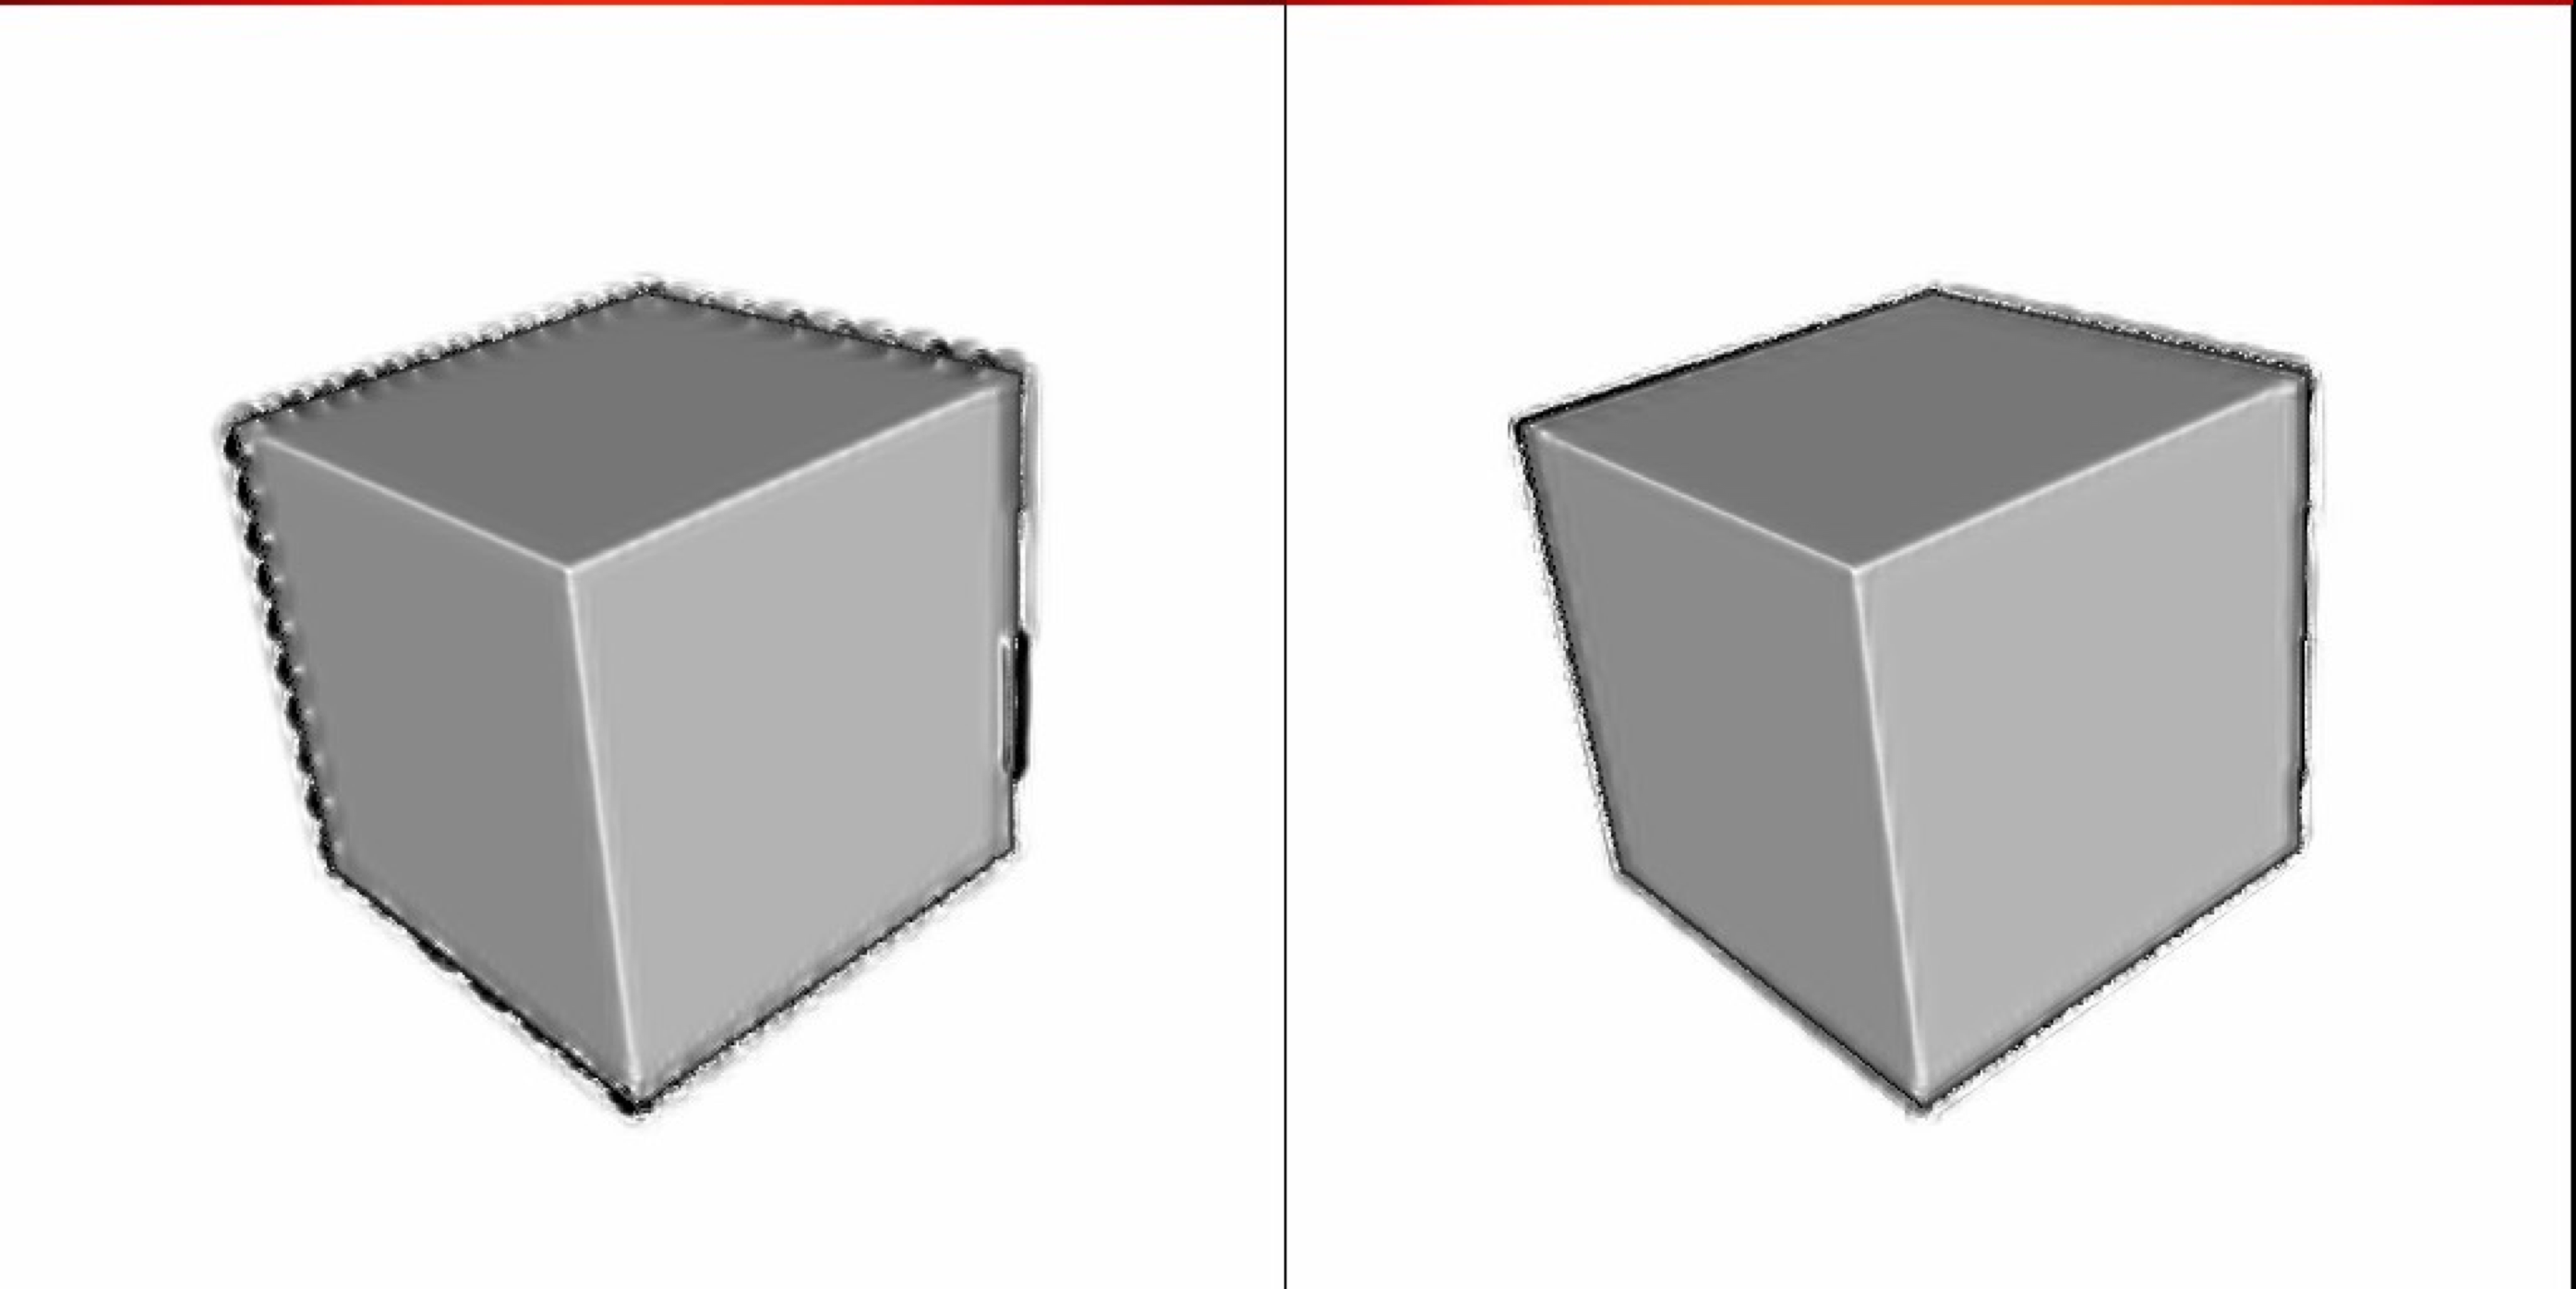
\includegraphics[width=0.45\columnwidth]{img/BadPix_failure.png}
%        \label{subfig:BadPix_fail}
%    } \\
%\end{tabular}

\caption{Results of upsampling using RMSE and related BadPix metrics can be visually poor. 
The top row shows the depth maps. The depth map with better upsampling  according to RMSE (left) could have severe visual distortions.
%Similarly, Figure~\ref{subfig:BadPix_fail} demonstrates that a number of bad pixels (threshold = 10)
%could appear on boundaries and depth discontuities, impairing the perceived
%quality of the result with higher BadPix (right).
}
\label{fig:datasets}
\end{center}
\end{figure}
\endgroup
% The \begingroup ... \endgroup pair ensures the separation
% parameters only affect this particular table, and not any
% sebsequent ones in the document.



In summary, our contributions are:
\begin{itemize}
    \item We demonstrate that RMSE and related measures do not capture   visual quality of 3D surface obtained from depth images compared to 
    specialized perceptually-based quality measures.
    \item We demonstrate that a simple perceptually-motivated metric for depth image comparison can be, on the one hand, easily combined with neural network-based whole-image upsampling techniques, and, on the other hand, is correlated with more complex perceptually based metrics.
    \item  We demonstrate with extensive comparisons, that two methods for depth image upsampling, one based on trained CNN architecture %trained on \TODO{what?} 
    and the other based on the deep image prior, yield high-quality results as measured by a number of perception-based metrics.
\end{itemize}

The rest of this paper is organized as follows. Section~\ref{sec:related} 
reviews the image-guided single depth image super-resolution problems
and literature on the visual metrics. In Section~\ref{sec:metrics},
we discuss our choice of the visually-based metrics used for training
and evaluation of the depth upsampling methods, 
and in Section~\ref{sec:methods} we summarize the methods themselves. Our computational experiments using a variety of datasets are described in Section~\ref{sec:exper} (the results are included as supplementary material).
